The goal of this work was to reconstruct some of the work of~\cite{GeneralIncremental15}, using their conecpt of a so-called Reactive Aggregator. More specifically, we wanted to develop a simple streaming aggregator for the ArgMax operator, based on that approach. Despite limiting our work to a bare minimum at the implementation level, we wanted to compare the results of the paper with the results that we get from our experiments.

Thus, our implementation is oriented after the original implementation architecture (see \autoref{fig:original_architecture}) which contains four main components:
\begin{description}
	\item[Windowing library:] processes the incoming data stream and informs the Reactive Aggregator about inserts, evicts or triggers (updates)
	\item[Reactive Aggregator:] handles the overall flow of the application, receiving events from the windowing library and pushing them to the FlatFAT object
	\item[FlatFAT:] contains all the intermediate results for the aggregation in a tree data structure, using the aggregation operations
	\item[Aggregation operations:] defining the neccessary implementation of the three functions lift, combine and lower for each specific aggregation operation (we only focus on the ArgMax aggregation operation)
\end{description}

\begin{figure}[H]
	\centering
	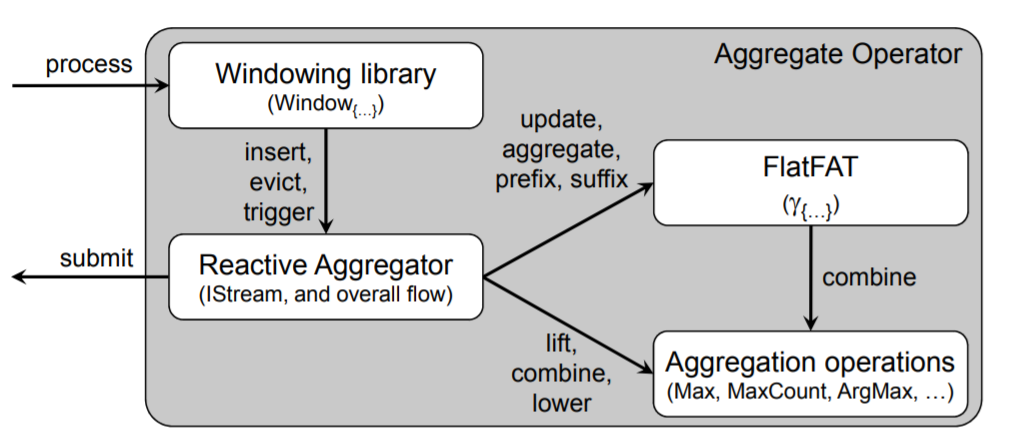
\includegraphics[width=\linewidth]{figures/original_architecture}
	\caption{Overview of the approach published in~\cite{GeneralIncremental15}}
	\label{fig:original_architecture}
\end{figure}